~\newpage
\nTitle{Programmation linéaire multicritère}

\section{Objectifs}
L'objectif est de trouver une solution de compromis entre les différents responsables.\\
Pour trouver une telle solution nous serons amenés à utiliser la programmation multicritère (\emph{PLM}).\\
~\\
Dans la première partie du rapport, nous avons trouvé un optimum pour chaque
responsable indépendam\-ment, ce qui nous conduit à un point de mire. Dans un
monde parfait, ce point de mire respecterait les contraintes de chaque
responsable. Nous devons donc voir si tel est le cas. 

\section{Recherche du point de départ}
Si le point de mire est assez proche de l'ensemble des solutions acceptables,
nous choisirons une solution proche de celle d'un responsable.

Sinon, nous allons calculer la satisfaction de chaque objectif, sachant qu'une
solution a été retenue. Nous devrons alors définir des métriques, correspondant
à cette satisfaction. Par exemple, pour le comptable, cette satisfaction sera
exprimée par le ratio du bénéfice obtenue dans un solution par rapport au
bénéfice maximal.
Ensuite, nous choisirons comme point de départ la solution qui offre le plus de
satisfaction à tout le monde, par exemple en utilisant une moyenne pondérée,
dont la pondération sera basée sur \emph{l'importance} de chaque critère.

\section{Affinement de la solution}
Les solutions trouvées précédemment peuvent certainement être optimisées. Il peut alors être
intéressant de \fg perdre\og dans un critère, si cela nous fait \og gagner\fg beaucoup dans
un autre critère, d'autant plus si ce second critère est jugé plus
\emph{intéressant} que le premier.

\section{Métriques utilisées}
Cette section décrit les métriques utilisées pour caractériser une solution, du
point de vue d'un cadre de l'entreprise. Les solutions pourront ainsi être
comparées entre elles.

\paragraph{Comptable :}
La métrique utilisée sera le pourcentage du bénéfice par rapport au bénéfice
maximum :
$$
M_{Comptable} = \frac{B_{S}}{B_{max}} \times 100
$$

\paragraph{Responsable d'atelier}
La métrique utilisée sera le pourcentage du nombre de produits fabriqués par
rapport au nombre maximum :
$$
M_{Atelier} = \frac{N_{S}}{N_{max}} \times 100
$$

\paragraph{Responsable des stocks}
Pour élaborer la métrique de satisfaction pour le responsable des stocks nous
opterons pour la fonction suivante, qui correspond à ce qui était précédemment
annoncé dans la partie 1 (page \pageref{sec:stocks}). 

\begin{figure}[!ht]
\begin{center}
    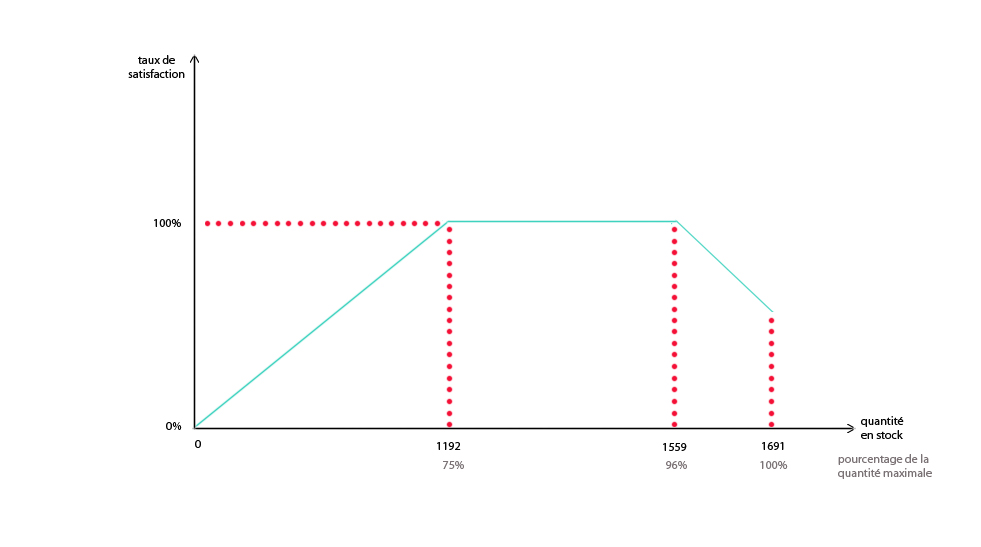
\includegraphics[width=13cm]{multicritere_graphe_stocks.png}
    \vspace{-1cm}
    \caption{Représentation graphique de la métrique pour le responsable des
	stocks.}
	\end{center}
\end{figure}

Cette fonction est décrite par l'expression suivante :
$$
M_{Stocks} = \left\{ 
    \begin{array}{l l l}
	\frac{x}{1192} \text{ si } x \in \text{[0 ; 1192]} \\
	x=1 \text{ si } x \in [1192 ; 1559]\\
	\frac{-x}{1192}+ 1+\frac{1559}{1192} \text{ si } x \in \text{[1559 ;
	    1691]}\\
    \end{array}
\right.
$$

Cette fonction pourrait être justifiée par le fait que plus on s’éloigne des
valeurs admises moins le responsable des stocks est satisfait. Les valeurs
numériques présentes dans la formules viennent des résultats de la section
\ref{sec:stocks} et sont visibles dans le graphique ci-dessous :


\paragraph{Responsable commercial}
La métrique utilisée sera l'écart par rapport à un équilibre parfait.
Si autant de produit de la famille de produit 1 (comprenant les produits A, B
et C) que de la famille 2 (comprenant les produits D, E et F), la métrique sera
à 100\%.
Si une seule famille de produit est fabriquée, la métrique devra valoir zéro.

Si $F_1$ (respectivement $F_2$ est le nombre de produit de la famille 1
(respectivement famille 2), la métrique sera :
$$
M_{Commercial} = \left( 1 - \frac{|F_1 - F_2|}{F_1 + F_2} \right) \times 100
$$

\section{Utilisation}
Les résultats seront placés dans un tableau de ce type, qui qui permettra d'un
seul coup d'œil de voir la meilleur des solutions. Ce tableau a été crée en
calculant les métrique pour chaque solution des quatre responsables.

La case en rouge se lira par exemple : 

\begin{center}
«~En suivant la volonté du responsable d'atelier, le comptable aura une
satisfaction de $96.5498\%$~»
\end{center}

    \begin{center}
	\begin{tabular}{|l|c|c|c|c|}
	    \hline
	    \cellcolor[gray]{0.9} & Comptable& Atelier & Stock & Commercial  \\
	    \hline
	    Comptable & 100.000\% & 94.7678\% & 88.9030\% & 11.4302\% \\
	    \hline
	    Atelier   & \cellcolor{red}96.5498\% & 100.000\% & 77.7846\% & 50.6491\% \\
	    \hline
	    Stock     & 74.1546\% & 70.8003\% & 99.9796\% & 0.00000\% \\
	    \hline
	    Commercial& 81.8653\% & 93.4330\% & 80.2626\% & 100.000\% \\
	    \hline
	\end{tabular}
    \end{center}

On voit déjà que la solution du commercial contente, dans une certaine mesure,
l'ensemble des responsables de l'entreprise, toutes les métriques sont
supérieures à 80\%.

\section{Optimisation}
Nous allons dans cette partie essayer de modifier les solutions précédentes
pour trouver une solution qui tente de maximiser la satisfaction des différents
responsables.

Le but premier d'une entreprise étant de faire du profit, et les meilleur 
manière de faire du profit étant souvent maximiser le bénéfice et d'avoir une
bonne politique commerciale, nous allons donc favoriser ces critères (bénéfice et
équilibrage des solutions), en leur appliquant un léger coefficient.

Nous allons par la même regarder l'évolution des autres critères lorsque ce
coefficient évolue, c'est à dire recalculer les différentes métriques.

Il apparaît plausible qu'avoir un \emph{stock non optimal} puisse être acceptable
si c'est pour avoir un bénéfice plus important, dans une certaine mesure. Une
dégradation de la satisfaction du responsable des stock sera donc moins
pénalisante, en terme de qualité de solution, qu'une baisse dans la satisfaction
du commercial (produire sans vendre ne sert pas à grand chose, en terme de
rentabilité).

De la même manière, produire un nombre de produit important peut être
intéressant, mais cela ne doit pas aller à l'encontre du profit et de la
mauvaise répartition de la production.

Nous pouvons donc donner des coefficients aux critères :

\begin{table}[h!]
\begin{center}
\begin{tabular}{|l||c|c|c|c|}
\hline
    Responsable & Comptable & Atelier &  Stocks & Commercial  \\
	\hline
    Coefficient & 1.2	    & 0.8     & 0.8	& 1.2 \\
	\hline
	\end{tabular}
	\end{center}
\caption{Coefficients associés aux critères des différents responsables}
\end{table}

Il faut cependant garder à l'esprit que ces coefficient devraient être ajustés
par une plus grande étude du cas spécifique d'\textbf{Optim}, les informations
dont nous disposons étant encore trop faibles pour effectuer une pondération
efficace.

\subsection{Méthodologie d'optimisation}
Le procédé est itératif, \textsl{i.e.} que nous allons, à chaque exécution de l'algorithme, nous rapproche,
de la solution, et tentera de contenter au mieux le comptable et le
commercial (comme expliqué ci-dessus).\\
~\\			  
Il s'agira donc de \textbf{partir de la solution du responsable commercial}
(celle qui dispose des taux de satisfaction les plus
haut), en essayant d'améliorer la métrique caractérisant la solution du
responsable comptable, tout en restant dans le domaines des solutions possibles
au vu des contraintes. Il faudra toutefois tâcher de ne pas trop dégrader les
autres critères.

Une solution serait de \emph{sacrifier} un peu d'équilibre dans les familles de
produit pour fabriquer des produits plus rentables. D'après la partie 1, section 
\ref{sec:comptable}, le produit qu'il faut fabriquer plus celui de type $E$.

\subsection{Résultats}
Etonnament, après le déroulement de l'aglorithme, les résultats n'ont pas apporté autant d'amélioration que prévu,
du fait de la faible latitude de changement des solutions, et parce que les produits en grande quantité dans la
famille 1 ne sont pas fait à partir des même matériaux que le produit à produire
dans la famille 2 (respectivement le produit $B$ et le produit $E$). Nous avion donc une solution \textsl{à priori} 
déjà proche d'un résultat optimal.\\
~\\
L'algorithme, assez naïf, essaie d'enlever un produit de la famille 1 pour
essayer de rajouter un produit de type $E$.

Ci dessous sont présenté les valeurs de satisfaction des quatre responsables ,
   en enlevant du produit de type $C$, et en rajoutant un produit de type $E$.

   Trois itérations sont possibles :
   \begin{table}[ht!]
   \begin{center}
\begin{tabular}{|c|c|c|c|c|}
\hline
    Itération & Comptable & Atelier & Stocks & Commercial \\
	\hline
1 &   81.9901 & 93.4330 & 30.6925 & 99.4319 \\
       \hline
2&   82.1148 & 93.4330 & 30.7764 & 98.8639 \\
       \hline
  3&  82.2396 & 93.4330 & 30.8603 & 98.2958 \\
       \hline

\end{tabular}
\end{center}
\caption{Résultats de l'exécution d'un algorithme d'optimisation}
\end{table}

\fbox{\textbf{Nous choisirons donc la solution 3, qui est la plus équilibrée, à partir de la
solution de départ que nous avons choisis.}}
